\chapter{Dane i analiza eksploracyjna}
\label{chap:eda}

\section{Źródło i struktura danych}

Dane wykorzystane w pracy pochodzą z publicznie dostępnej kolekcji zbiorów danych zebranych przez zespół Juliana McAuleya~\cite{mcauleySteamData} z Uniwersytetu Kalifornijskiego w San Diego w celu budowy systemów rekomendacyjnych i personalizacji. W szczególności wykorzystano podzbiór zawierający biblioteki gier użytkowników platformy dystrybucji cyfrowej Steam.

Źródłowe dane miały postać pliku JSON, w którym każdy rekord opisywał bibliotekę jednego użytkownika, identyfikowanego przez zmienną \texttt{user\_id}. Dla każdego użytkownika dostępna była lista przypisanych do niego gier wraz z identyfikatorem gry (\texttt{item\_id}), nazwą (\texttt{item\_name}) oraz łącznym czasem rozgrywki (\texttt{playtime\_forever}) w minutach. Dane wejściowe zostały przekształcone do postaci ramki danych, w której pojedynczy wiersz odpowiada unikalnej parze użytkownik--gra.

\section{Dane jako niejawna informacja zwrotna}

Wykorzystane dane nie zawierają jawnych ocen przypisanych przez użytkowników, takich jak wartości liczbowe lub gwiazdki. Jedynymi sygnałami behawioralnymi informującymi o~relacji użytkownika z~grą są jej obecność w~bibliotece oraz łączny czas rozgrywki. Zatem rekomendacje będą oparte na zmiennej \texttt{playtime\_forever}, która pełni rolę miary intensywności relacji między danym użytkownikiem i produktem. Z tego powodu jest to problem rekomendacji na podstawie niejawnej informacji zwrotnej. Warto podkreślić, że jest to silnie zaszumiony sygnał i jego wartość nie odzwierciedla proporcjonalnie zainteresowania danym tytułem~\cite{hu2008implicit}. Stanowi to motywację do badania wpływu przekształceń tej zmiennej na jakość rekomendacji.

\section{Podstawowe statystyki surowego zbioru}

Podstawowe statystyki surowego zbioru zestawiono w~tabeli~\ref{tab:raw_data_basic_stats}. Przed filtracją analizowany zbiór zawierał 5\,153\,209 interakcji, obejmujących 70\,912 użytkowników oraz 10\,978 gier. Wynika stąd, że obserwowana macierz użytkownik--gra była bardzo rzadka: jej gęstość wynosiła około 0{,}00662, co oznacza, że zaobserwowane zostało zaledwie 0{,}662\% wszystkich możliwych interakcji w macierzy. Niska gęstość macierzy jest powszechna w dziedzinie systemów rekomendacyjnych, ponieważ przeciętny użytkownik wchodzi w~interakcję z~niewielkim ułamkiem katalogu liczącego tysiące lub miliony pozycji.

\begin{table}[htbp]
\centering
\caption{Podstawowe statystyki surowego zbioru danych}
\label{tab:raw_data_basic_stats}
\begin{tabular}{lr}
\toprule
Statystyka & \multicolumn{1}{c}{Wartość} \\
\midrule
Liczba interakcji użytkownik--gra & 5\,153\,209 \\
Liczba użytkowników & 70\,912 \\
Liczba gier & 10\,978 \\
Gęstość macierzy & 0{,}00662 \\
\bottomrule
\end{tabular}
\end{table}

\section{Wpływ przygotowania danych na strukturę zbioru}

Przed treningiem i ewaluacją modeli dane zostały poddane filtracji. Szczegółowy opis i uzasadnienie tych decyzji przedstawiono w rozdziale~\ref{chap:metodologia}. W tym podrozdziale omówiono jedynie ich wpływ na rozmiar oraz strukturę finalnego zbioru, zestawiony w~tabeli~\ref{tab:data_preparation_effect}.

\begin{table}[htbp]
\centering
\caption{Wpływ kolejnych etapów przygotowania danych na rozmiar zbioru}
\label{tab:data_preparation_effect}
\begin{tabular}{lrrr}
\toprule
Etap & \multicolumn{1}{c}{Interakcje} & \multicolumn{1}{c}{Użytkownicy} & \multicolumn{1}{c}{Gry} \\
\midrule
Dane surowe & 5\,153\,209 & 70\,912 & 10\,978 \\
Po filtracji gier & 5\,149\,512 & 70\,912 & 9\,198 \\
Po filtracji użytkowników & 5\,132\,610 & 62\,944 & 9\,198 \\
\bottomrule
\end{tabular}
\end{table}

Usunięto 20\,599 interakcji, co odpowiada około 0{,}40\% początkowego zbioru. Jednocześnie liczba użytkowników zmniejszyła się o~7\,968, czyli o~11{,}24\%, a~liczba gier o~1\,780, czyli o~16{,}21\%. Gęstość macierzy użytkownik--gra wzrosła z~0{,}00662 do około 0{,}00887, jednak nadal pozostała bardzo niska. Zatem zbiór po przygotowaniu nadal ma charakter rzadkich danych rekomendacyjnych, ale jest mniej obciążony przypadkami o~małej liczbie interakcji.

Dysproporcja między odsetkiem usuniętych interakcji a~odsetkiem usuniętych obiektów wskazuje, że filtracja objęła przede wszystkim gry występujące u~pojedynczych użytkowników oraz konta o~znikomej historii. Dla takich przypadków wyznaczenie reprezentacji w~przestrzeni czynników ukrytych jest utrudnione. Rekomendacje dla użytkowników o~kilku interakcjach opierałyby się w~praktyce na rozkładzie popularności, a~gry obecne w~pojedynczych bibliotekach miałyby małą szansę pojawić się na listach rekomendacyjnych, obniżając przy tym pokrycie katalogu. Należy jednak zaznaczyć, że filtracja sprowadza zbiór do gęstszej postaci, ułatwiając tym samym zadanie rekomendacyjne. Przyjęte progi mogą zatem wpływać na wartości uzyskiwanych metryk oraz na wnioski płynące z~porównania modeli.

\section{Rozkład czasu gry i interakcje z zerowym czasem gry}

Istotną cechą analizowanego zbioru jest występowanie interakcji, dla których wartość zmiennej \texttt{playtime\_forever} wynosi zero. Oznacza to, że dana gra znajduje się w bibliotece użytkownika, ale nie odnotowano żadnego czasu rozgrywki. Interakcje z~zerowym czasem gry stanowiły 36{,}25\% wszystkich obserwacji w~przygotowanym zbiorze. Usunięcie ich z~analizy zmieniłoby definicję problemu, ponieważ model uczyłby się wyłącznie na podstawie gier faktycznie uruchomionych, pomijając znaczną liczbę obserwacji pozytywnych. Sama obecność gry w~bibliotece stanowi bowiem sygnał behawioralny świadczący o~zainteresowaniu tytułem. W pracy obserwacje z \texttt{playtime\_forever = 0} zostały zachowane jako poprawne interakcje użytkownik--gra. Nie jest to podejście standardowe, ponieważ w~pracach poświęconych danym z~tej platformy rekordy bez zarejestrowanego czasu gry bywają usuwane~\cite{bunga2021implicit, cheuque2019steam}. Świadome odejście od tej praktyki wynika z chęci uniknięcia utraty ponad jednej trzeciej danych oraz zachowania sygnału intencji zakupu, który z punktu widzenia analizy preferencji konsumenckich wciąż niesie ze sobą istotną wartość informacyjną.

Dla interakcji z dodatnim czasem gry rozkład zmiennej \texttt{playtime\_forever} jest silnie prawostronnie skośny. Większość obserwacji koncentruje się przy stosunkowo niskich wartościach, a duże czasy rozgrywki tworzą długi ogon. Na rysunku~\ref{fig:filtered_positive_playtime_hist} przedstawiono histogram dodatnich wartości czasu gry w skali logarytmicznej.

\begin{figure}[htbp]
    \centering
    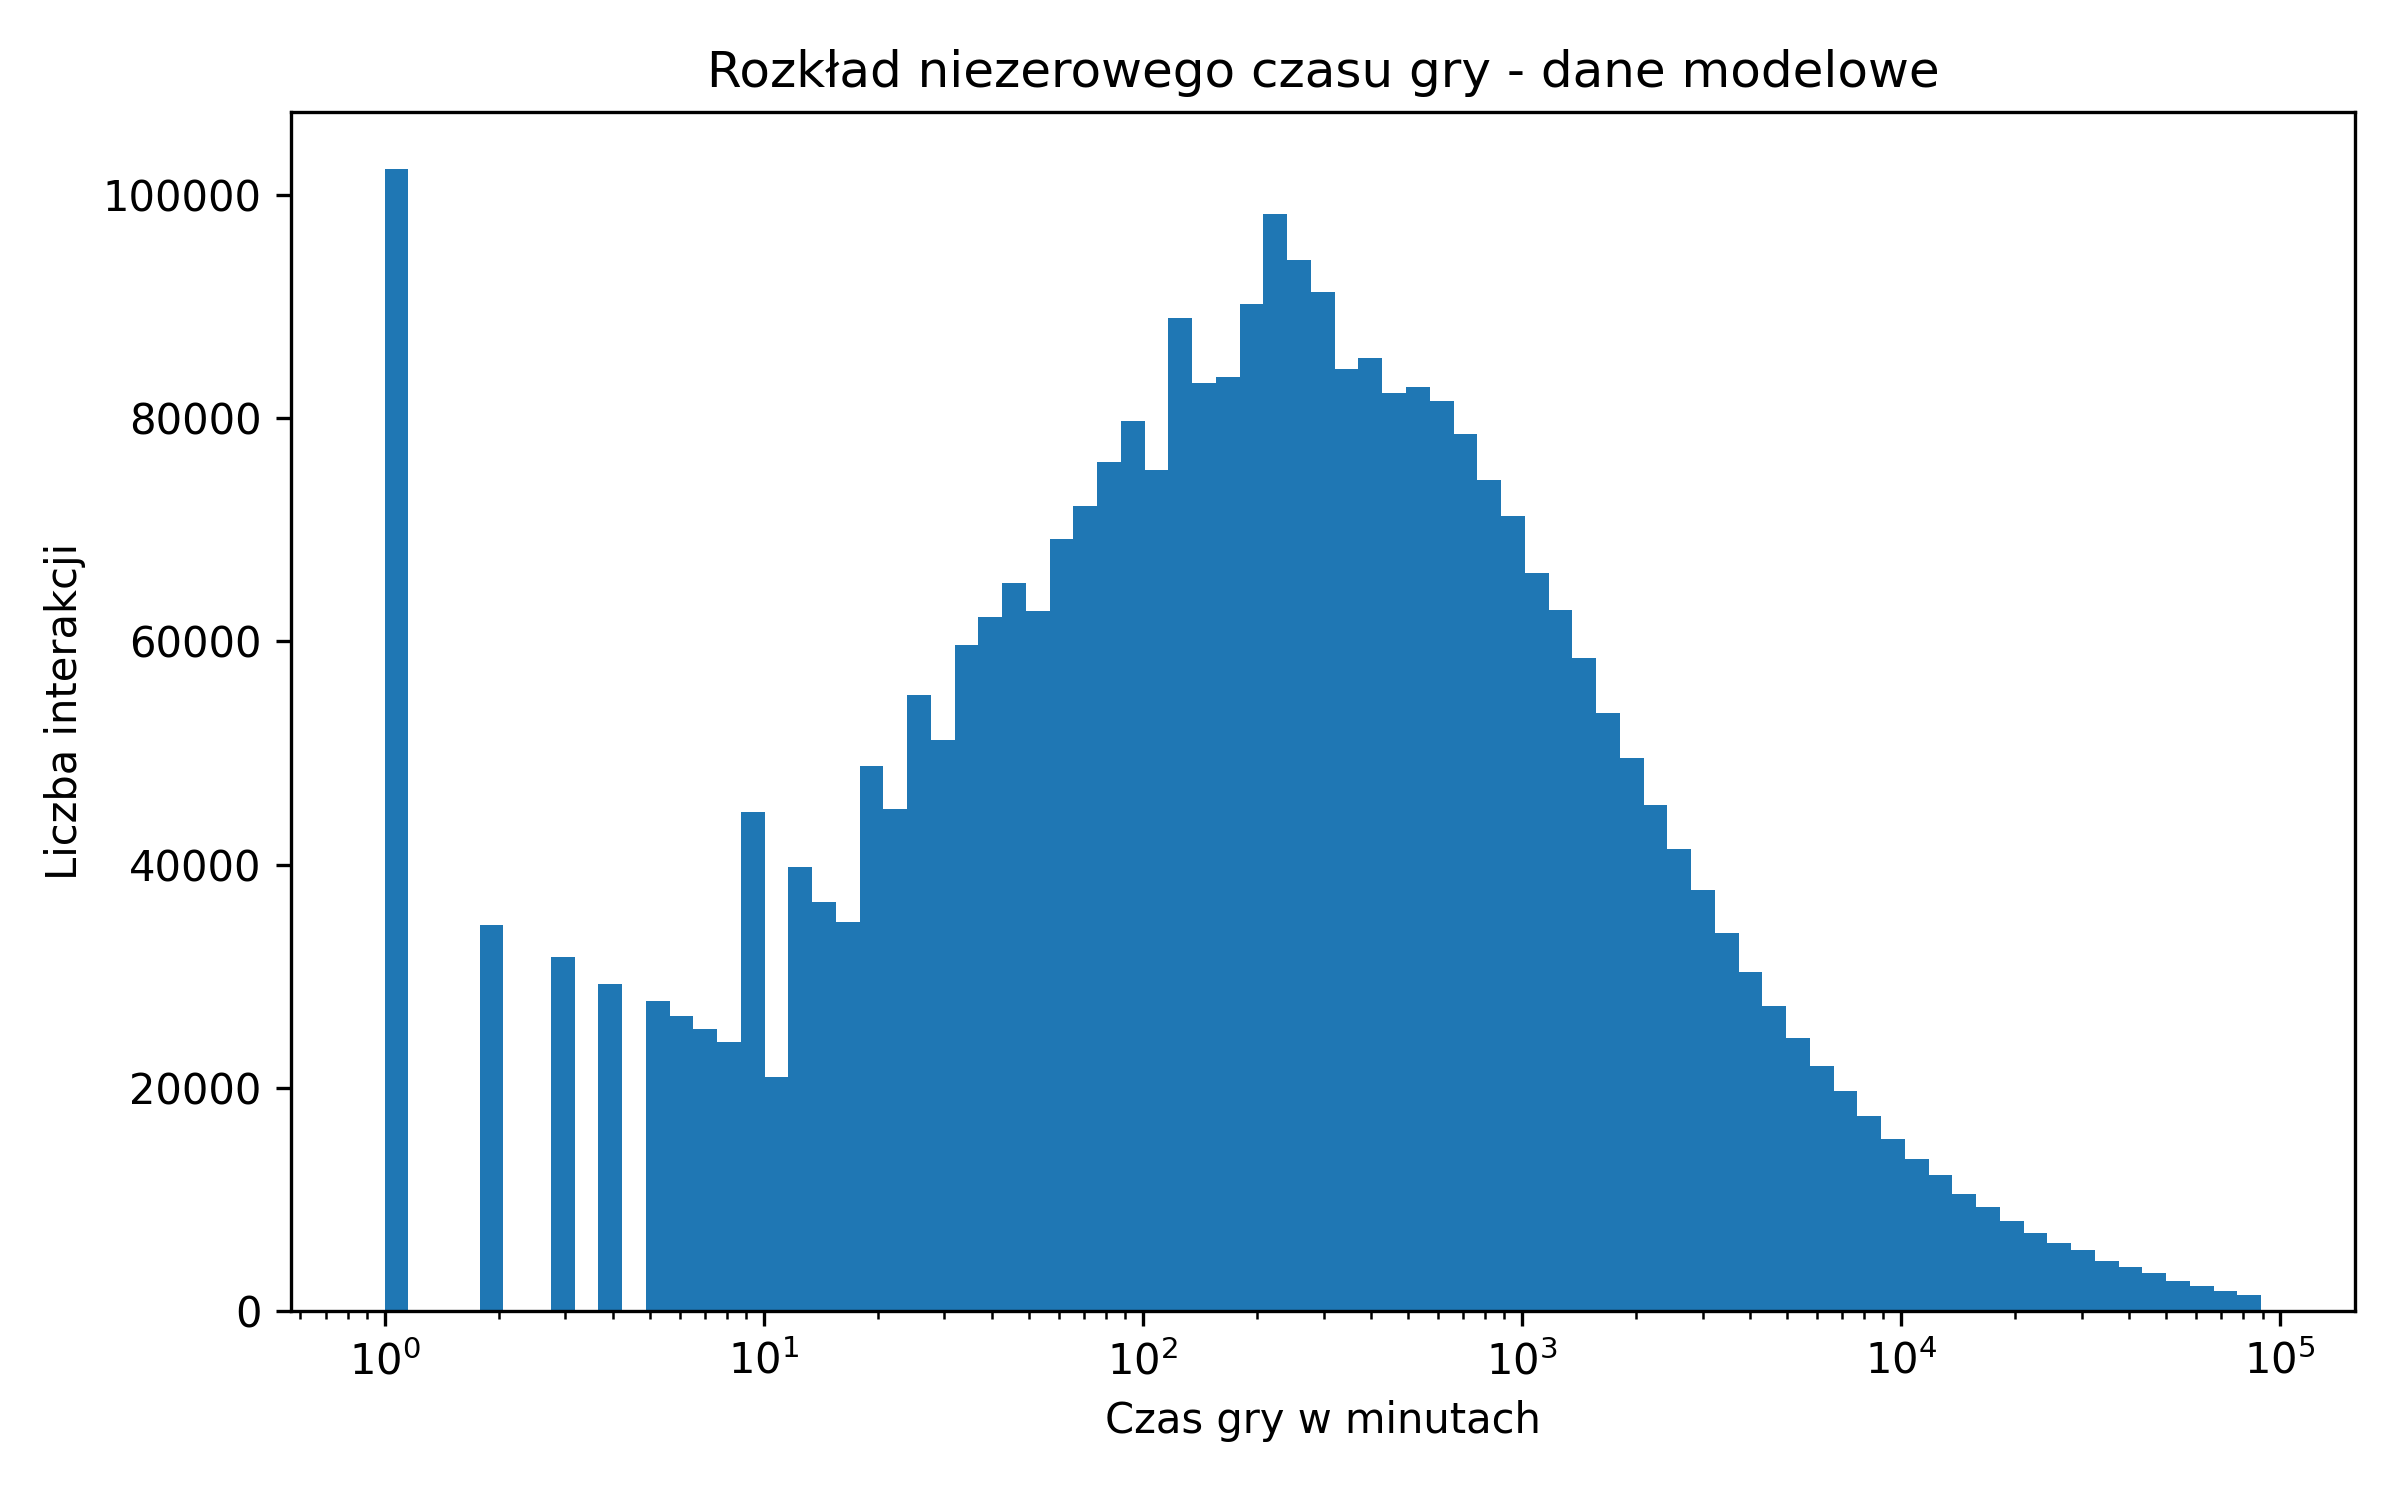
\includegraphics[width=0.9\textwidth]{figures/eda/filtered/filtered_positive_playtime_logscale_hist.png}
    \caption{Rozkład dodatniego czasu gry w skali logarytmicznej w przygotowanym zbiorze}
    \label{fig:filtered_positive_playtime_hist}
\end{figure}

Skośność rozkładu czasu gry stanowi przesłankę do rozważenia funkcji pewności o~spowolnionym wzroście. Liniowe potraktowanie zmiennej \texttt{playtime\_forever} nadawałoby bardzo dużą wagę skrajnym obserwacjom, przez co mogłoby zaburzać proces uczenia modelu. Natomiast sam fakt obecności gry w bibliotece pozostaje istotną informacją nawet wtedy, gdy czas gry jest równy zero. Z tego powodu w pracy zbadane zostały funkcje pewności ograniczające wpływ skrajnych wartości zmiennej odpowiadającej za czas gry oraz nadające obserwacjom z zerowym czasem gry zwiększoną wagę bazową. Definicje poszczególnych funkcji pewności przedstawiono w~podrozdziale~\ref{sec:porownywane-modele}.

\section{Aktywność użytkowników i popularność gier}

\subsection{Aktywność użytkowników}

Rozkład liczby interakcji przypadających na użytkownika jest prawostronnie
skośny, co przedstawiono na rysunku~\ref{fig:filtered_user_interaction_counts}. Widoczne skupienie przy niskich wartościach oraz długi ogon pokazują, że zbiór łączy dużą liczbę użytkowników o umiarkowanej aktywności z niewielką grupą kont posiadających bardzo rozbudowane biblioteki. W przygotowanym zbiorze średnia liczba interakcji na użytkownika wynosiła 81{,}54, podczas gdy mediana była równa 48. Pełne zestawienie statystyk rozkładu przedstawiono w~tabeli~\ref{tab:user_item_activity_stats}.

\begin{table}[htbp]
\centering
\caption{Rozkład liczby interakcji użytkowników i popularności gier w przygotowanym zbiorze}
\label{tab:user_item_activity_stats}
\begin{tabular}{lrr}
\toprule
Statystyka & \multicolumn{1}{c}{Na użytkownika} & \multicolumn{1}{c}{Na grę} \\
\midrule
Średnia & 81{,}54 & 558{,}01 \\
Mediana & 48 & 71 \\
95. percentyl & 251 & 2\,515{,}05 \\
99. percentyl & 518{,}57 & 8\,811{,}84 \\
Maksimum & 7\,337 & 45\,699 \\
\bottomrule
\end{tabular}
\end{table}

\begin{figure}[htbp]
    \centering
    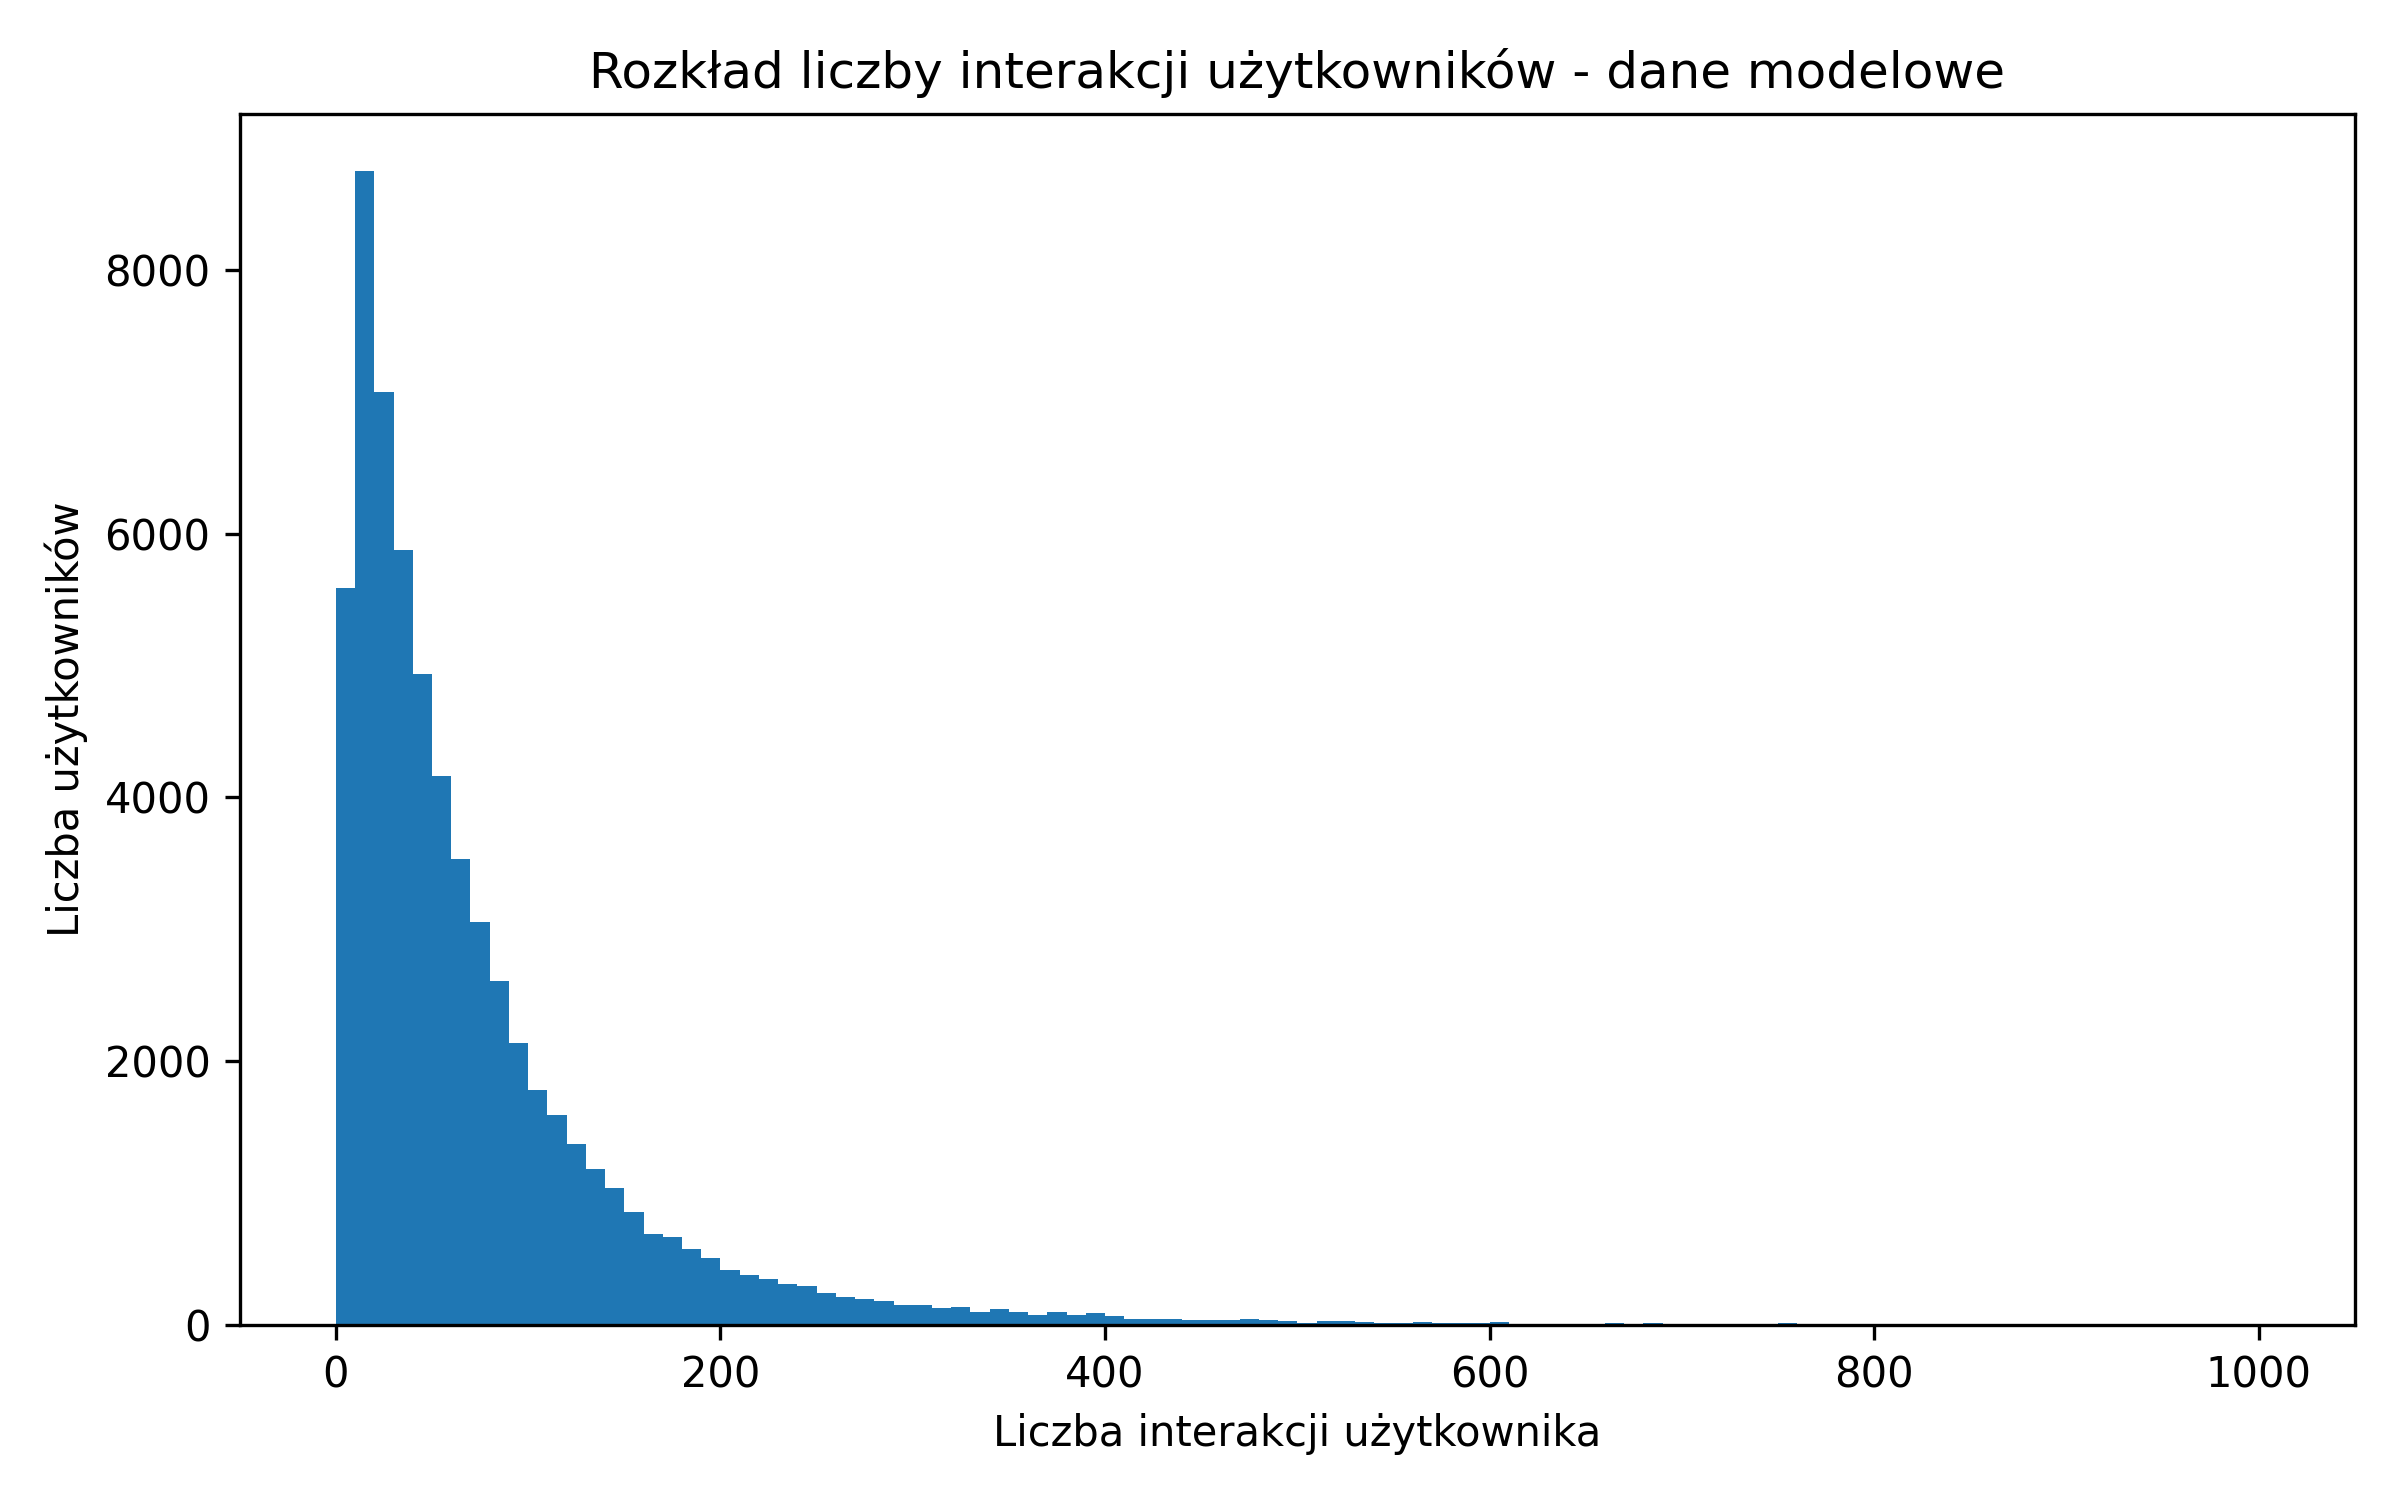
\includegraphics[width=0.9\textwidth]{../results/eda/figures_filtered/filtered_user_interaction_counts_hist.png}
    \caption{Rozkład liczby interakcji przypadających na użytkownika w przygotowanym zbiorze danych}
    \label{fig:filtered_user_interaction_counts}
\end{figure}

\subsection{Popularność gier}

Jeszcze większe zróżnicowanie widać po stronie gier. Mediana liczby interakcji przypadających na grę wynosiła 71, podczas gdy średnia była równa 558{,}01. Wynika stąd, że większość gier występowała w~bibliotekach stosunkowo małej liczby użytkowników, natomiast niewielka grupa najpopularniejszych tytułów odpowiadała za bardzo dużą część wszystkich interakcji.

Koncentrację popularności przedstawiono na rysunku~\ref{fig:filtered_item_popularity_concentration}. Najpopularniejszy 1\% gier odpowiadał za około 27{,}16\% wszystkich interakcji, najpopularniejsze 5\% za 59{,}55\%, a najpopularniejsze 10\% za 74{,}71\%.

\begin{figure}[htbp]
    \centering
    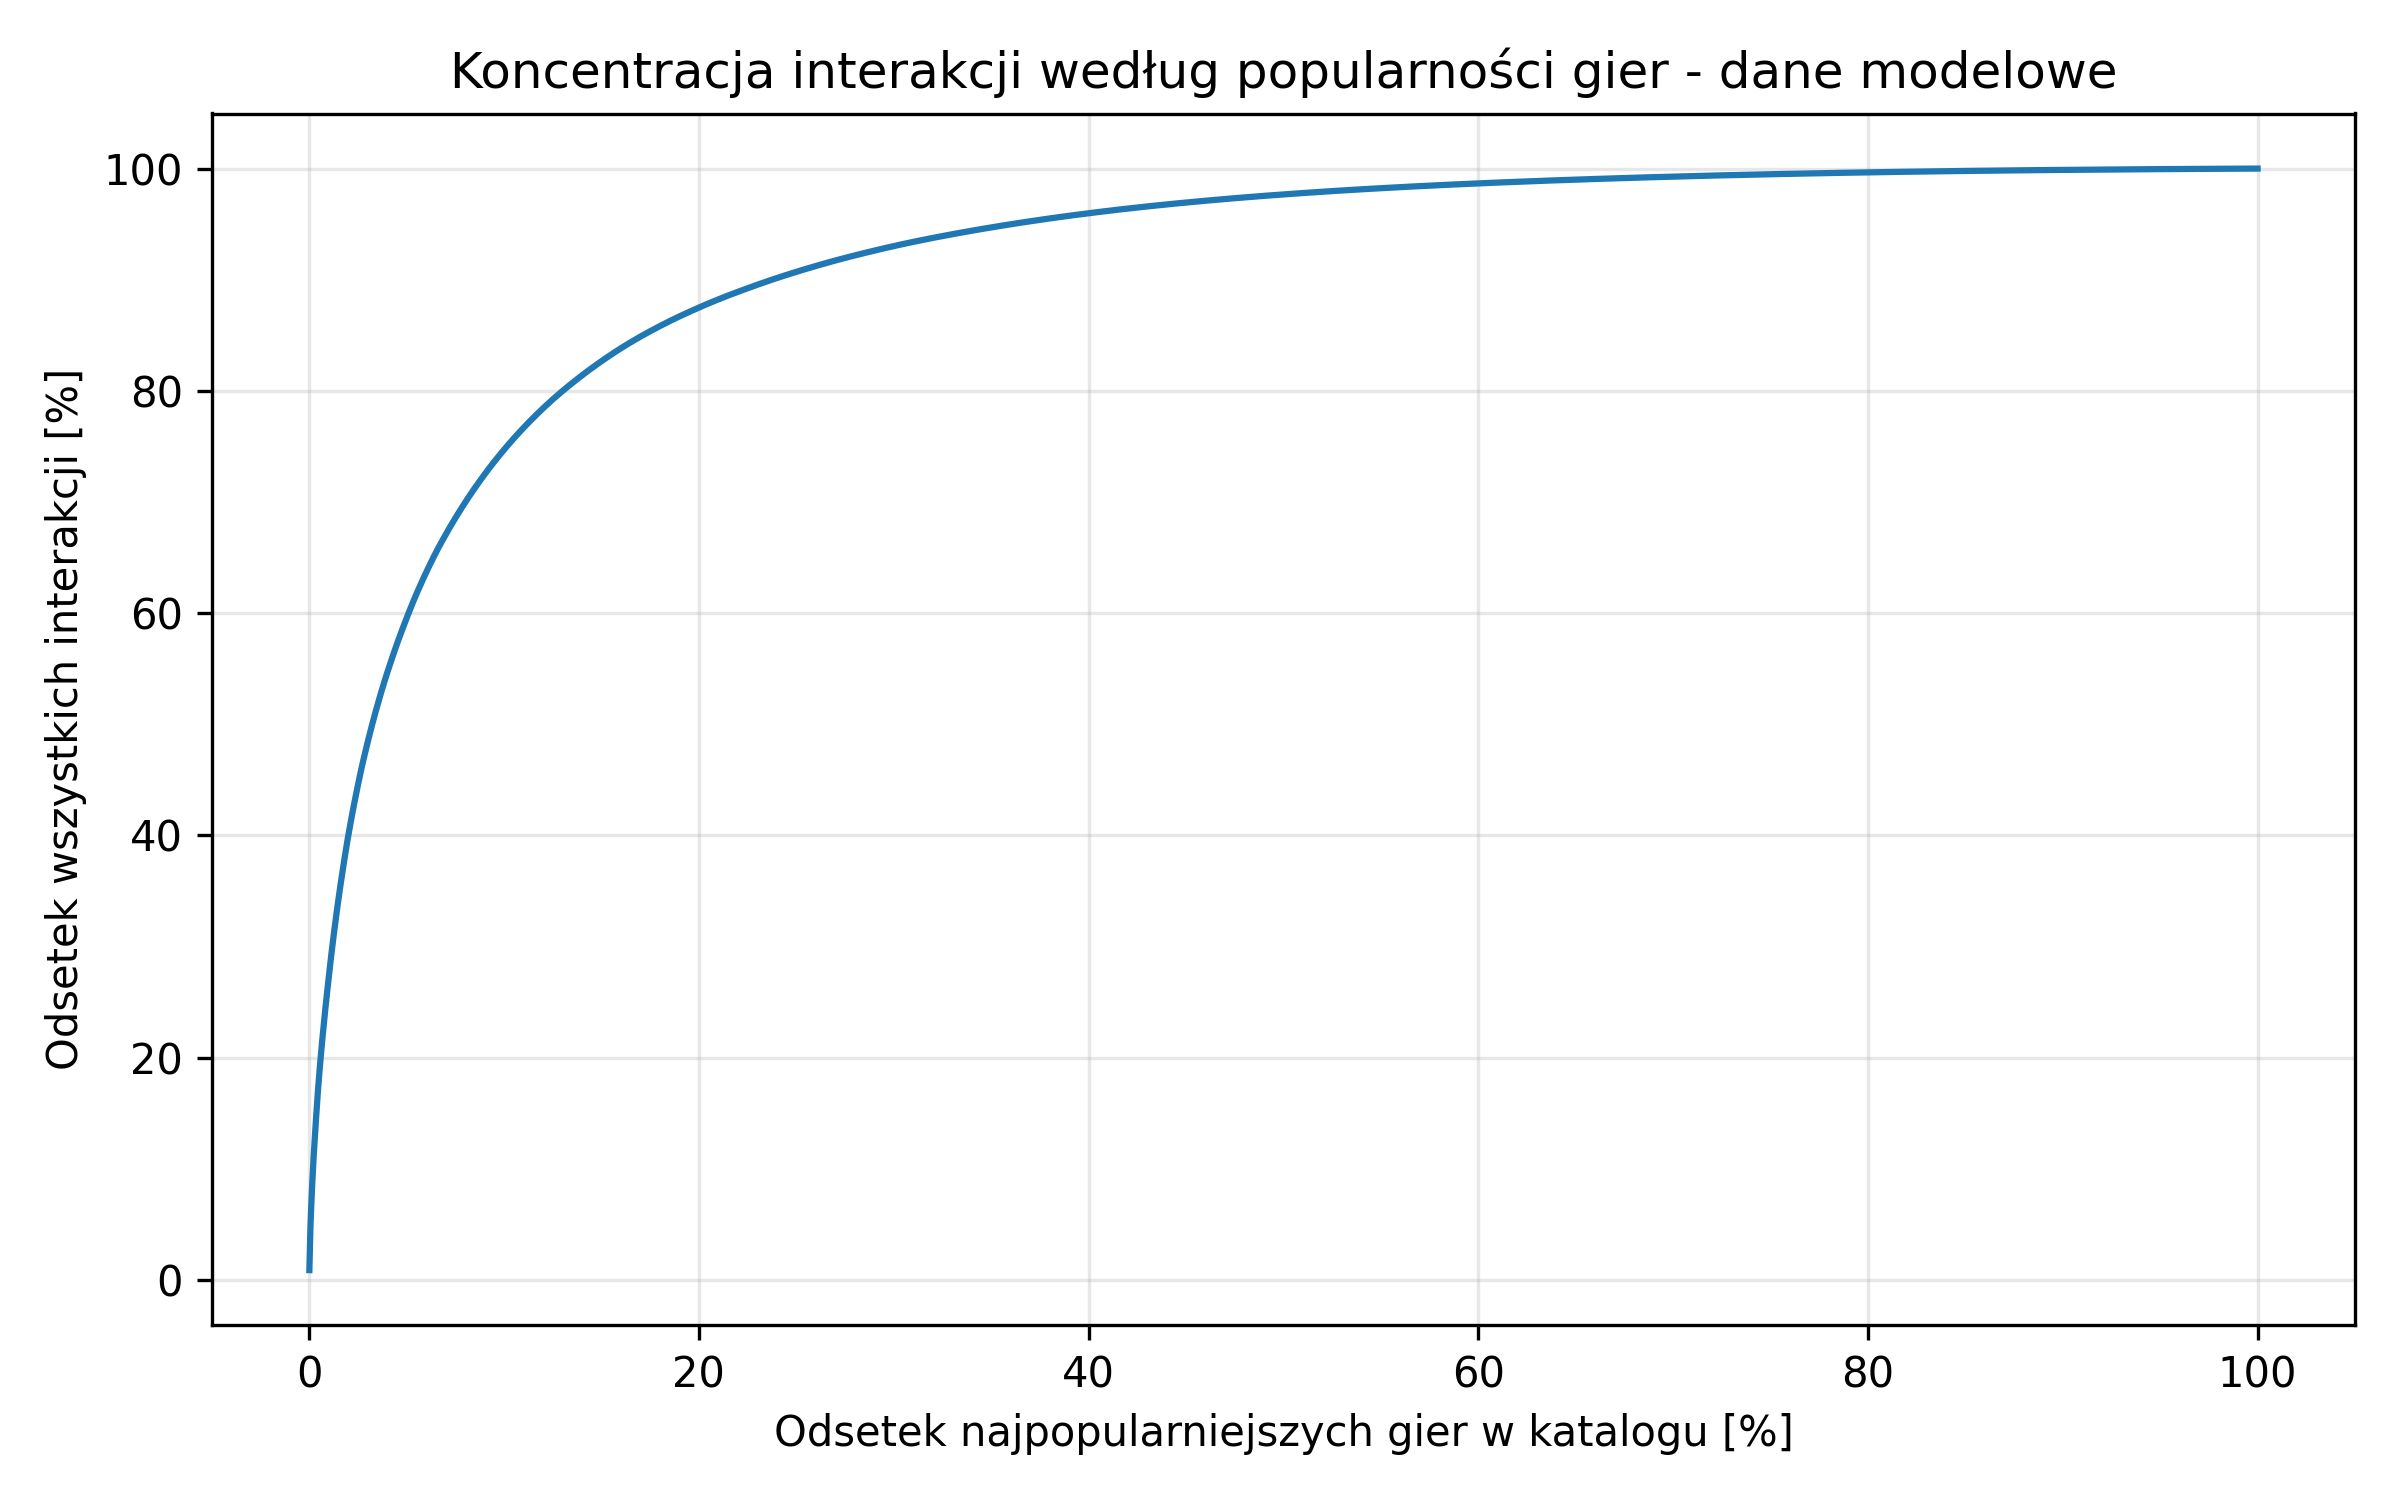
\includegraphics[width=0.9\textwidth]{../results/eda/figures_filtered/filtered_item_popularity_concentration.png}
    \caption{Koncentracja interakcji według popularności gier w przygotowanym zbiorze danych}
    \label{fig:filtered_item_popularity_concentration}
\end{figure}

Dodatkową ilustracją tej nierównomierności jest zestawienie najpopularniejszych gier przedstawione na rysunku~\ref{fig:filtered_top_games}. Wśród tytułów o największej liczbie interakcji znajdują się przede wszystkim bardzo popularne gry wieloosobowe oraz darmowe produkcje obecne w bibliotekach dużej liczby użytkowników. Obecność takich pozycji pokazuje, że prosty model oparty wyłącznie na popularności mógłby generować pozornie atrakcyjne rekomendacje, ale jednocześnie silnie ograniczałby różnorodność katalogu.

\begin{figure}[htbp]
    \centering
    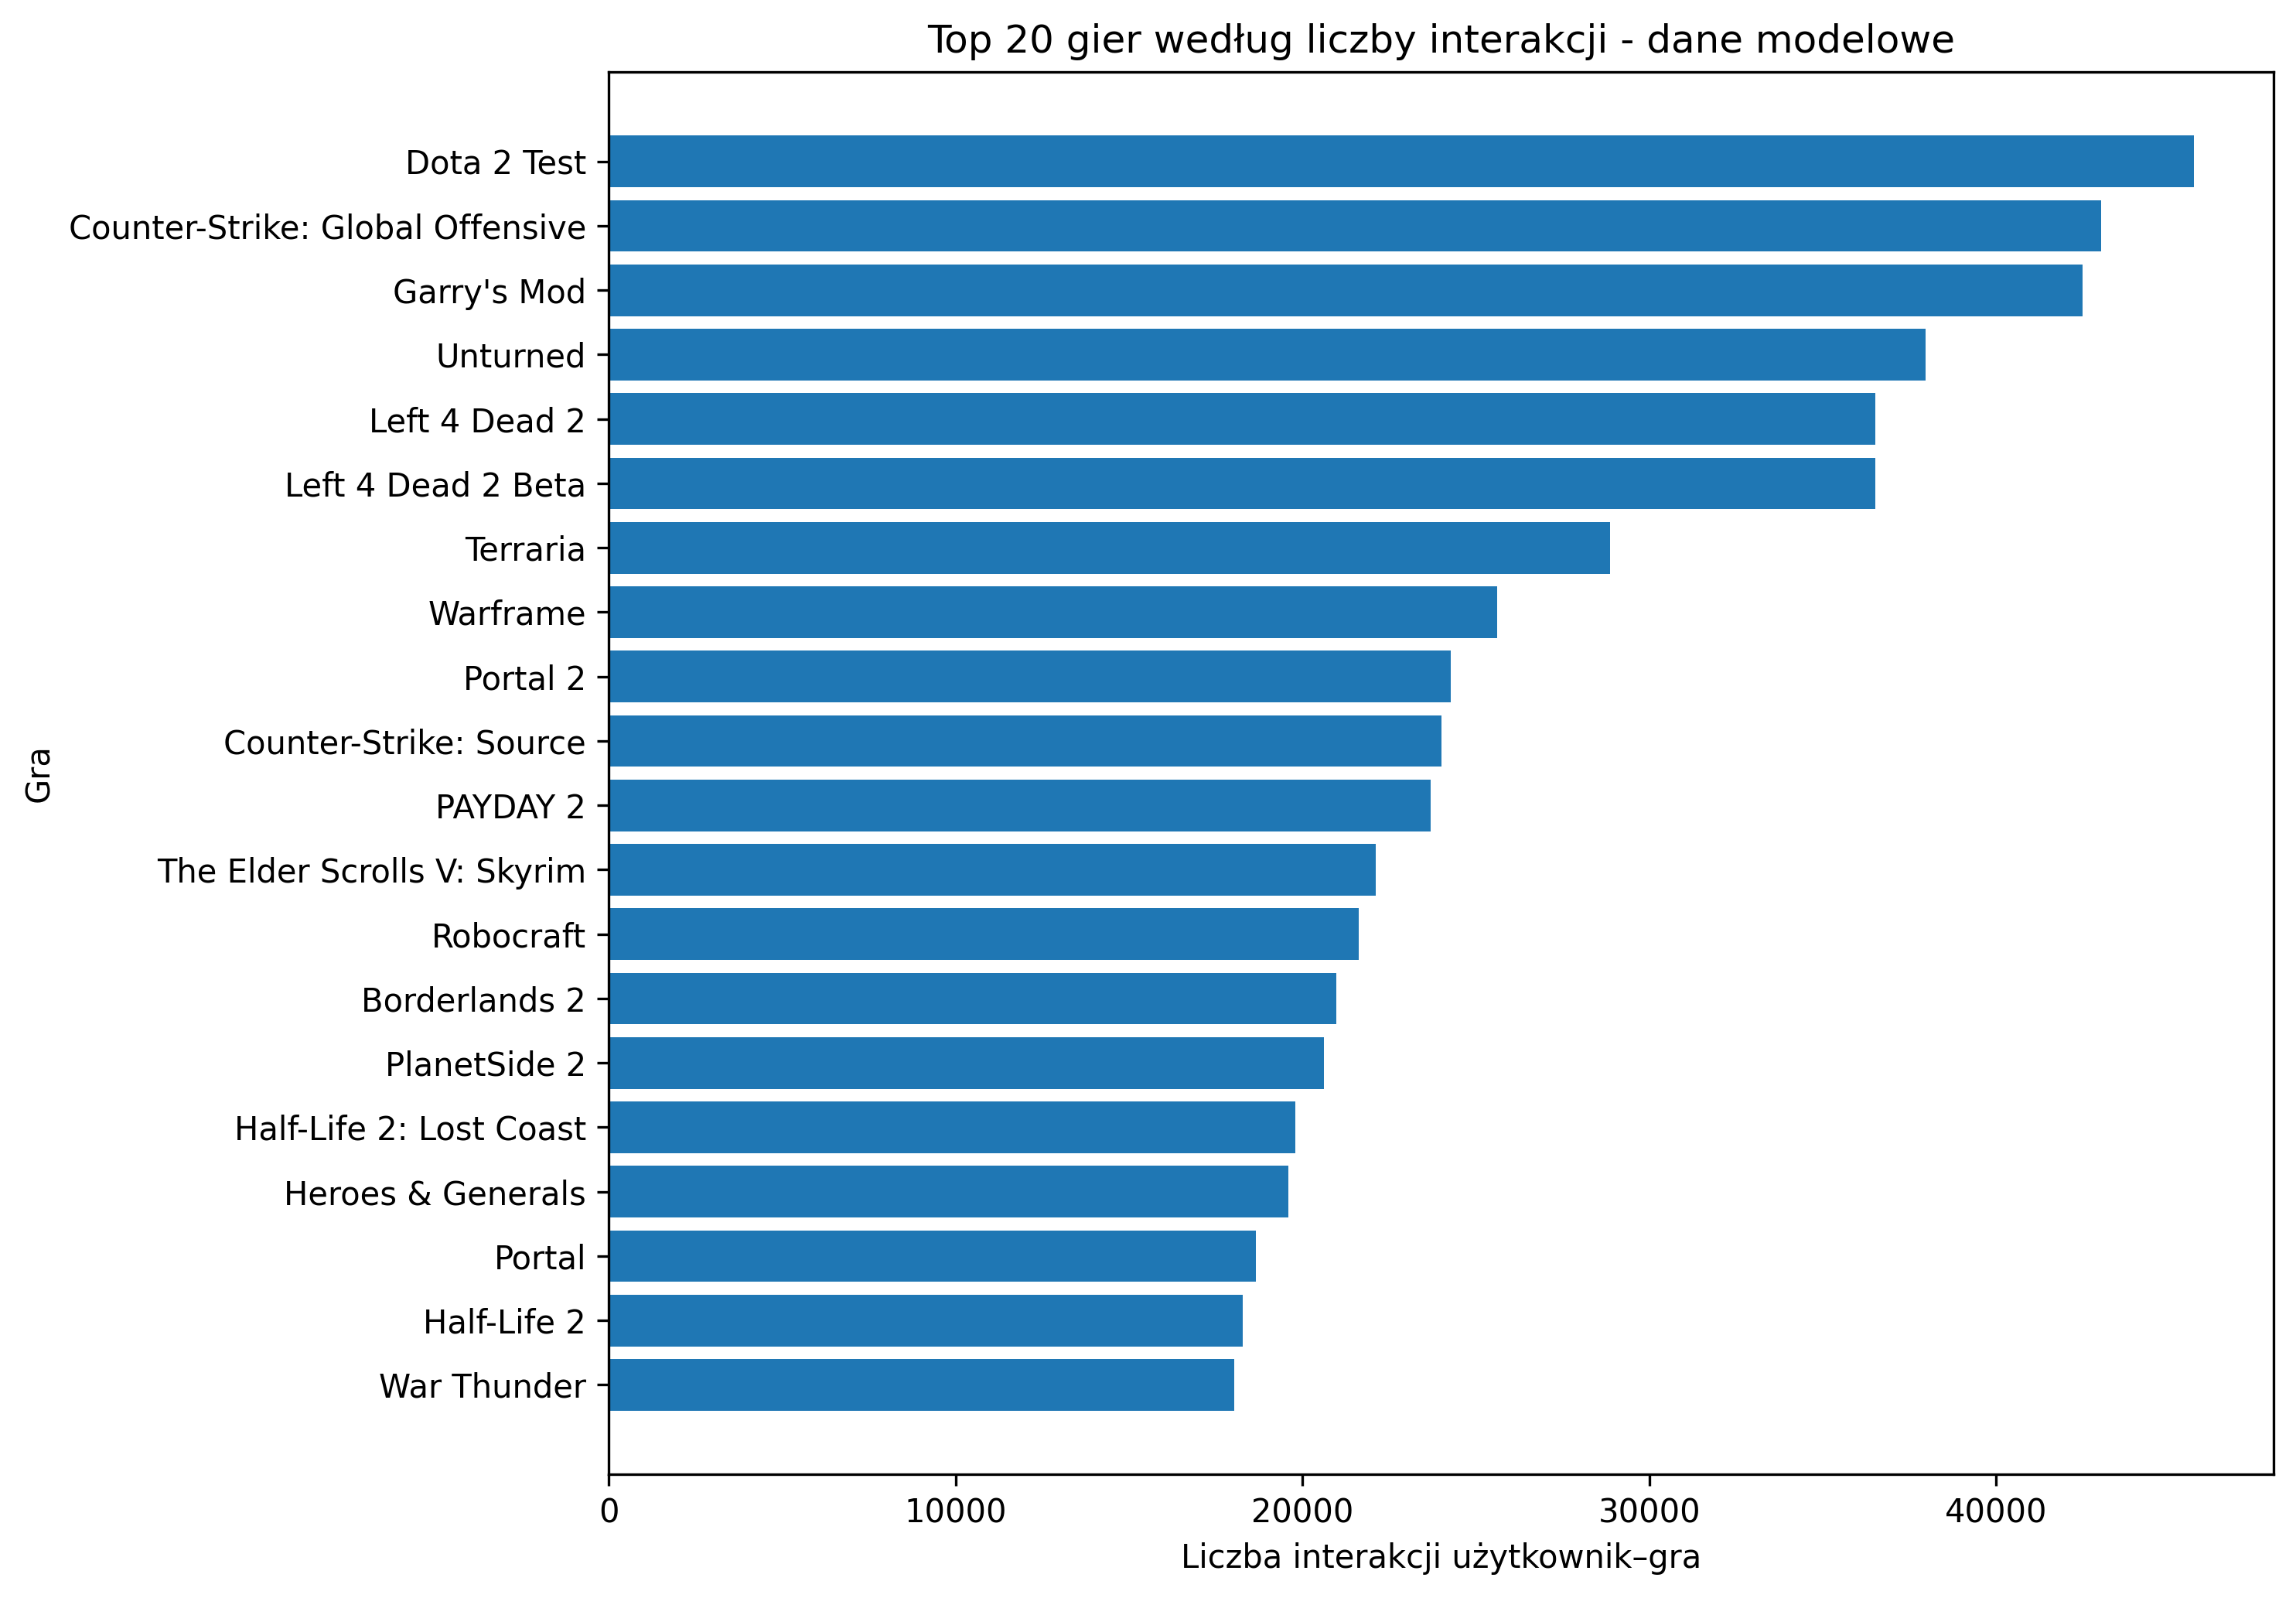
\includegraphics[width=0.9\textwidth]{../results/eda/figures_filtered/filtered_top_20_games_by_interactions.png}
    \caption{Dwadzieścia najpopularniejszych gier według liczby interakcji w przygotowanym zbiorze danych}
    \label{fig:filtered_top_games}
\end{figure}

Zaobserwowana koncentracja popularności ma znaczenie dla interpretacji późniejszych wyników eksperymentalnych. Modele rekomendacyjne mogą osiągać dobrą trafność, często rekomendując najpopularniejsze tytuły, ale takie zachowanie prowadzi do niskiego pokrycia katalogu i silnego obciążenia rekomendacji popularnością. Z tego powodu w dalszej części pracy, obok metryk trafności rankingowej, analizowane są również miary pokrycia katalogu oraz popularności rekomendowanych gier~\cite{kaminskas2016diversity,abdollahpouri2019unfairness}.

\section{Wnioski z analizy eksploracyjnej}

Najważniejsze cechy analizowanego zbioru danych, które bezpośrednio wpłynęły na przyjętą metodologię badawczą, to silnie prawostronnie skośny rozkład czasu gry użytkowników oraz wyraźna koncentracja popularności gier. Rozkład zmiennej \texttt{playtime\_forever} charakteryzuje się długim ogonem, co wymaga odpowiedniego przekształcenia tej zmiennej w wagę pewności wykorzystywaną w modelu. Z kolei nierównomierny rozkład popularności gier oznacza, że niewielka część katalogu generuje znaczną część interakcji, co należy uwzględnić w ocenie jakości rekomendacji poprzez analizę miar pokrycia katalogu oraz obciążenia popularnością.

Kolejnym istotnym aspektem jest rola obserwacji z wartością \texttt{playtime\_forever = 0}, które odmiennie od dominującego w literaturze trendu ich usuwania~\cite{bunga2021implicit, cheuque2019steam} zostały zachowane w procesie uczenia jako istotny sygnał behawioralny. Ich uwzględnienie wymaga funkcji pewności, która przypisuje takim obserwacjom wagę podwyższoną względem wartości domyślnej. Osobną kwestią pozostaje, czy jednoczesne spowolnienie przyrostu wagi dla rosnących czasów gry poprawia jakość rekomendacji. Odpowiedź na to pytanie przedstawiono w~dalszej części pracy.